%!TeX root=main.tex
\chapter{شبکه 
	\lr{LXMERT}}
\thispagestyle{empty}
استدلال در ترکیب تصویر و زبان نیاز به فهم بصری، فهم زبانی و ارتباط مابین فهم بصری و فهم زبانی دارد. شبکه 
\lr{LXMERT}
\LTRfootnote{\lr{Language Cross-Modality Encoder Representation from Transformers}}
 برای حل مسئله‌های زبانی-بصری طراحی شده است. 
\lr{LXMERT}
  یک شبکه عصبی از قبل آموزش دیده 
\LTRfootnote{\lr{pretrain}}
از نوع ترنسفورمر می‌باشد که بر خلاف ترنسفورمرهای معمول از 3 رمزگذار
\LTRfootnote{\lr{encoder}}
 تشکیل می‌شود. در ادامه درباره معماری شبکه، ساختار رمزگذار و نحوه آموزش اولیه
 \LTRfootnote{\lr{pretrain}}
  شبکه توضیحاتی داده می‌شود \cite{tan2019lxmert}.


\section{معماری شبکه}
	همان‌طور که در شکل \ref{lxmert-arc} قابل مشاهده است، شبکه
	\lr{LXMERT}
	از لایه‌های 
	\lr{self-attention}
	و 
	\lr{cross-attention}
	تشکیل شده است. یک تصویر و جمله مرتبط با آن به عنوان ورودی به شبکه داده می‌شود. هر تصویر شامل دنباله‌ای از 
	\lr{object}
	می‌باشد. شبکه
	\lr{LXMERT}
	بازنمایی مناسبی از تصویر و زبان و 
	\lr{cross-modality}
	ایجاد می‌کند.


\begin{figure}
	\center{\includegraphics[width=0.9\linewidth]{images/lxmert-arc.PNG}}
	\caption{معماری شبکه \lr{LXMERT} \cite{tan2019lxmert}}
	\label{lxmert-arc}
\end{figure}

\subsection{ورودی شبکه}
ورودی شبکه
\lr{LXMERT}
از دو بخش
\lr{Word-Level Sentence Embedding}
و 
\lr{Object-Level Image Embeddings}
تشکیل شده است.

در بخش
\lr{Word-Level Sentence Embedding}
جملات توسط 
\lr{WordPiece tokenizer}
به توکن‌هایی جدا می‌شوند. در ادامه هر توکن توسط لایه
\lr{embedding}
به بردار بازنمایی تبدیل می‌شود. مشابه شبکه
\lr{BERT}\cite{devlin-etal-2019-bert}
برای نمایش محل دقیق توکن در جمله از
\lr{Index Embedding}
استفاده می‌شود.

در بخش 
\lr{Object-Level Image Embeddings}
به جای استفاده از
\lr{CNN's feature map}
، ویژگی‌های پیدا شده توسط 
\lr{Faster-RCNN}\cite{ren15fasterrcnn}
مورد استفاده قرار می‌گیرد.

\subsection{رمزگذارهای شبکه}
شبکه
\lr{LXMERT}
شامل
\lr{Language Encoder}،
\lr{Object-relationship Encoder}
و
\lr{Cross-modality Encoder}
می‌باشد. هر رمزگذار از 
\lr{self-attention}
و 
\lr{cross-attention}
تشکیل شده است.

\subsubsection{\lr{Attention Layers}}
مشابه مکانیزم توجه
\LTRfootnote{\lr{Attention}}
در ترنسفورمر می‌باشد. توضیحات دقیق‌تر در بخش \ref{attention} داده شده است.

\subsubsection{رمزگذار
	\lr{Single-Modality}}
بعد از لایه 
\lr{embedding}
برای هر کدام از ورودی‌های زبان و تصویر دو رمزگذار
\LTRfootnote{\lr{encoder}}
مجزا وجود دارد. محاسبات در این دو رمزگذار از یکدیگر مستقل هستند. هر رمزگذار شامل مکانیزم توجه
\LTRfootnote{\lr{Attention}}
و شبکه 
\lr{Feed Forward}
%\LTRfootnote{\lr{Feed Forward}}
می‌باشد. همچنین بعد از هر زیر لایه اتصال رو به جلو
\LTRfootnote{\lr{residual connection}}
و لایه نرمال‌سازی
\LTRfootnote{\lr{normalization layer}}
 وجود دارد که با نماد "+" در شکل
\ref{lxmert-single-encoder}
 نشان داده شده است.

\begin{figure}[H]
	\center{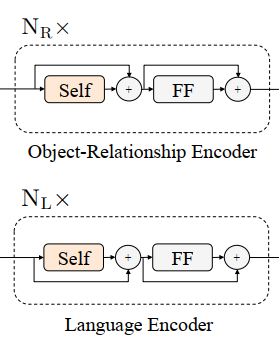
\includegraphics[width=0.5\linewidth]{images/single-encoder.PNG}}
	\caption{رمزگذار 
		\lr{Single-Modality} 
		در شبکه
		\lr{LXMERT} \cite{tan2019lxmert}}
	\label{lxmert-single-encoder}
\end{figure}
\subsubsection{رمزگذار
	\lr{Cross-Modality}}

\subsection{خروجی شبکه}
خروجی شبکه
\lr{LXMERT}
از سه بخش تصویر، زبان و 
\lr{cross-modality}
تشکیل می‌شود. بخش زبان و تصویر توسط رمزگذار
\lr{Cross-Modality}
و با توجه به دنباله ورودی هر مورد تولید شده است. خروجی 
\lr{cross-modality}
از توکن 
\lr{CLS}
تشکیل شده و کاربردی همانند آنچه در 
\lr{BERT}
ذکر شده دارد.
\section{استراتژی آموزش اولیه 
%	\lr{Pre-Training}
}
\subsection{ روش‌های آموزش اولیه}

%\LTRfootnote{\lr{ Pre-Training}}
شبکه 
\lr{LXMERT}
به طور کلی توسط سه نوع روش
\lr{pre-train}
می‌شود. در ادامه توضیحی مختصری از هر روش آورده شده است.
\begin{figure}[H]
	\center{\includegraphics[width=0.9\linewidth]{images/pretraining-lxmert.PNG}}
	\caption{مثالی از آموزش اولیه
	شبکه
	 \lr{LXMERT} \cite{tan2019lxmert}}
	\label{lxmert-pretrain}
\end{figure}
\subsubsection{\lr{Language Task: Masked Cross-Modality LM }}
در این روش همچون روشی که در شبکه
\lr{BERT}
استفاده شده، پانزده درصد توکن‌های ورودی با توکن
\lr{Mask}
جایگزین می‌شوند. فرق اجرا این روش در 
\lr{LXMERT}
با 
\lr{BERT}
در این است که در 
\lr{BERT}
تشخیص توکن
\lr{Mask}
تنها با استفاده از توکن‌های جمله ورودی انجام می‌شود. این در حالی است که در 
\lr{LXMERT}
علاوه بر توکن‌های جمله ورودی، از ویژگی‌های تصویر هم در تشخیص توکن
\lr{Mask}
استفاده می‌شود. همان‌طور که در شکل 
\ref{lxmert-pretrain}
قابل مشاهده است، در صورتی که کلمه
\lr{Carrot}
برای 
\lr{Mask}
شدن انتخاب شود،
وجود تصویر در تشخیص درست شبکه برای کلمه 
\lr{Mask}
شده از اهمیت بالایی برخوردار است.
\subsubsection{\lr{Vision Task: Masked Object Prediction}}
مشابه قسمت زبانی، در این قسمت نیز بخشی از ویژگی ورودی تصویر
\lr{Mask}
می‌شود و شبکه به کمک جمله مرتبط با تصویر و سایر ویژگی‌های تصویر که
\lr{Mask}
نشده‌اند، قسمت مورد نظر را تشخیص می‌دهد. با توجه به نوع ورودی‌ها در این روش همچون روش قبلی مدل
\lr{cross-modality alignment}
را نیز فرا می‌گیرد. 

\subsubsection{\lr{Cross-Modality Task}}
برای آموزش بهتر بخش 
\lr{cross-modality}
از دو روش دیگر نیز استفاده شده است.
\begin{enumerate}
	\item روش \lr{Cross-Modality Matching}
	
هر جمله به احتمال 50 درصد با یک جمله نامرتبط با تصویر جایگزین می‌شود. سپس یک رده‌بند\LTRfootnote{\lr{classifier}}
آموزش داده می‌شود تا مطابقت تصویر و جمله را بررسی کند. این مسئله شبیه به پیشبینی جمله بعدی \LTRfootnote{\lr{Next Sentence Prediction}}
در آموزش اولیه شبکه 
\lr{BERT}
می‌باشد.

	\item روش \lr{Image Question Answering}
	
در این روش یک تصویر و سوال مرتبط با تصویر داده می‌شود و وظیفه مدل پیش‌بینی پاسخ می‌باشد.
\end{enumerate}

\subsection{مجموعه داده استفاده شده در آموزش اولیه}
برای آموزش اولیه از 5 مجموعه داده استفاده شده است که شامل 
\lr{COCO-Cap}،
\lr{VG-Cap \LTRfootnote{\lr{Visual Genom Caption}}}،
\lr{VQA \LTRfootnote{\lr{Visual Question Answering}}}،
\lr{GQA \LTRfootnote{\lr{A New Dataset for Real-World Visual Reasoning and Compositional Question Answering}}}
و
\lr{VG-QA \LTRfootnote{\lr{Visual Genom - Question Answering}}}
می‌باشد. فقط از مجموعه آموزشی
\LTRfootnote{\lr{Train}}
و ارزیابی
\LTRfootnote{\lr{Dev}}
مجموعه داده‌های فوق استفاده شده است. برای هر تصویر چندین پرسش و پاسخ موجود است.

\subsection{نتایج}
	در نهایت  دقت این شبکه بر روی 3 مجموعه داده 
	\lr{NLVR}
	،
	\lr{VQA}
	و
	\lr{GQA}
	مورد بررسی قرار گرفته است. در هر سه مورد نتایج نسبت به
	\lr{State Of The Art}
	بهبود قابل توجهی داشته است (شکل
	\ref{lxmert-result}).
	\begin{figure}[H]
		\center{\includegraphics[width=0.8\linewidth]{images/LXMERT-result.PNG}}
		\caption{نتایج شبکه 
			\lr{LXMERT}\cite{tan2019lxmert}}
		\label{lxmert-result}
	\end{figure}